% !TEX root = main.tex

\section{Decay-time Resoution}
\label{sec:Resolution}

The observed oscillation of B mesons is prone to dilution, if the detector resolution is of similar magnitude as the oscillation period. 
In the \Bs system, considering that the measured oscillation frequency of the \Bs \cite{PDG2014} and the average LHCb detector resolution \cite{LHCb-DP-2014-002} are both $\mathcal{O}(50 \fs^{-1})$, this is the case.
Therefore, it is crucial to correctly describe the decay time resolution in order to avoid a bias on the measurement of time dependent CP parameters. \newline
In the presented analysis, we assume a gaussian resolution function with different widths for each event. 
This gives rise to a per-event decay time error $\sigma_{t}$, which is computed separately for every event along with the proper time $t$, by the decay time fitter. 
Furthermore, the per-event decay time error $\sigma_{t}$ is usualy underestimated by the decay time fitter, 
making it necessary to derive a scaling function, which matches the per-event error to the actually measured decay time resolution. \newline

Due to the lack of a decay time unbiased sample of real $\Bs\to\Ds\kaon\pion\pion$ decays, this analysis relies on simulation to describe the time resolution. 
The obtained results will be compared to those found in the closely related $\Bs\to\Ds\kaon$ analysis and systematic uncertainties will be assigned conservatively.
In the following, we investigate the Run1 and Run2 MC samples to find the proper decay time resolution in bins of the per-event decay time erros and derive a scaling function from that.      

\subsection{Formalism} 

For simulated $\Bs\to\Ds\kaon\pion\pion$ events, the information on the true $\Bs$ lifetime $\tau_{true}$ assigned at production of the event, 
as well as the measured decay time $\tau_{measured}$, which is determined after the interaction with the LHCb detector, is stored. 
In this analysis, the difference $\Delta t = \tau_{true} - \tau_{measured}$ is obtained for each simulated $\Bs\to\Ds\kaon\pion\pion$ candidate. 
The width of the distribution of $\Delta t$ is a direct measure of the decay time resolution. \newline 
To analyse the relation between the per-event decay time eror $\sigma_{t}$ and the actual resolution, the simulated sample is split into 8 bins of $\sigma_{t}$. 
Each bin width is chosen using an adaptive binnning scheme which ensures that approximately equal numbers of events are found in every bin.  
A fit is then performed to the distribution of $\Delta t$ in each of the bins to determine the decay time resolution in the respective bin. 
After that, the correlation between the binned per-event decay time error and the measured decay time resolution is analyzed to determine the scaling function.     


\subsection{Decay-time Error in Run I \& Run II}

Due to the increase in center of mass energy from Run I to Run II, as well as (among others) new tuning in the patern and vertex reconstruction, 
the distributions of the raw decay time error might no necessarily match each other between the two different runs. 
Significant deviations can be observed in the shape and mean of those two distributions for $\Bs\to\Ds\kaon\pion\pion$ signal candidates shown in Figure \ref{fig:Bs_DTFERR_Comp}.

\begin{figure}[h]
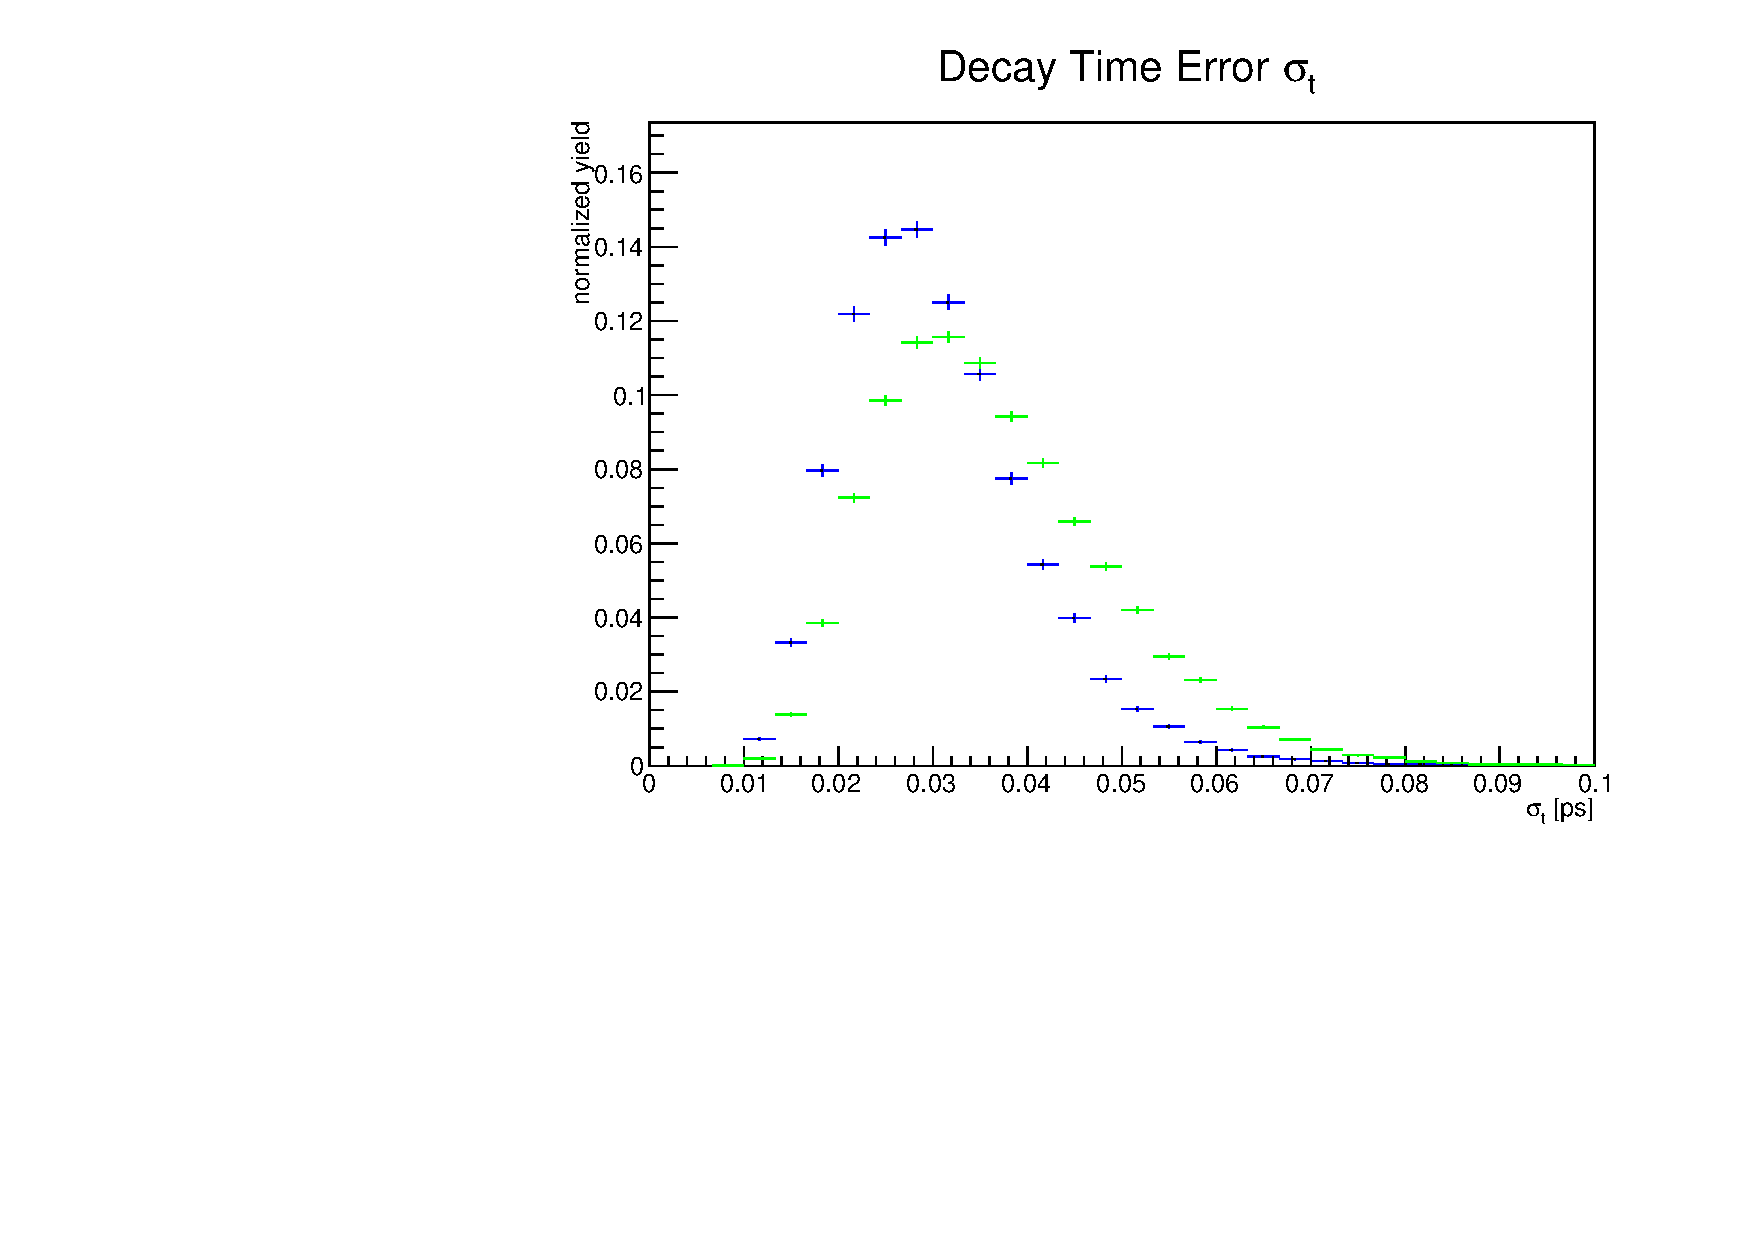
\includegraphics[height=7.4cm,width=0.7\textwidth]{figs/Resolution/Bs_DTFERR_runComp.pdf}
\caption{Distribution of the decay time error for $\Bs\to\Ds\kaon\pion\pion$ signal candidates on data for (blue) Run I and (green) Run II. The signal distributions are obtained using the sWeight technique.}
\label{fig:Bs_DTFERR_Comp}
\end{figure}

It can be observed that the decay time error distribution for signal cadidates from Run II is significantly broader and shifted to slightly hihger values.
Due to the discrepancies between the distributions of the decay time error $\sigma_{r}$ for Run I and Run II data, the time resolution studies have to be performed seperately for both runs, 
which leads to two different scaling functions to map $\sigma_{t} \to \sigma_{eff}$. 


\subsection{Fits to the decay time distributions}

The sum of two Gaussian functions is used to fit the distributions of the decay time difference $\Delta t$ in each $\sigma_{t}$ bin.
One Gaussian function is relatively narrow and describes the decay time of the majority of candidates in each bin, 
while the other, broader Gaussian function describes candidates where the measure decay time differs considerably from $\tau_{true}$. 
Those contributions are shifted to the tails of the distribution. From the two Gaussian functions, the combined, effective width $\sigma_{eff}$ is quoted as decay time resolution in each bin. 
Figure \ref{fig:ResoFit_24to29} shows the double Gaussian fit to the distirbution of the decay time difference for events where $20.7\ps$ $<$ $\sigma_{t}$ $<$ $24.3\ps$. 
All fits are shown in the Appendix \ref{subsec:DecResFits}. \newline

\begin{figure}[h]
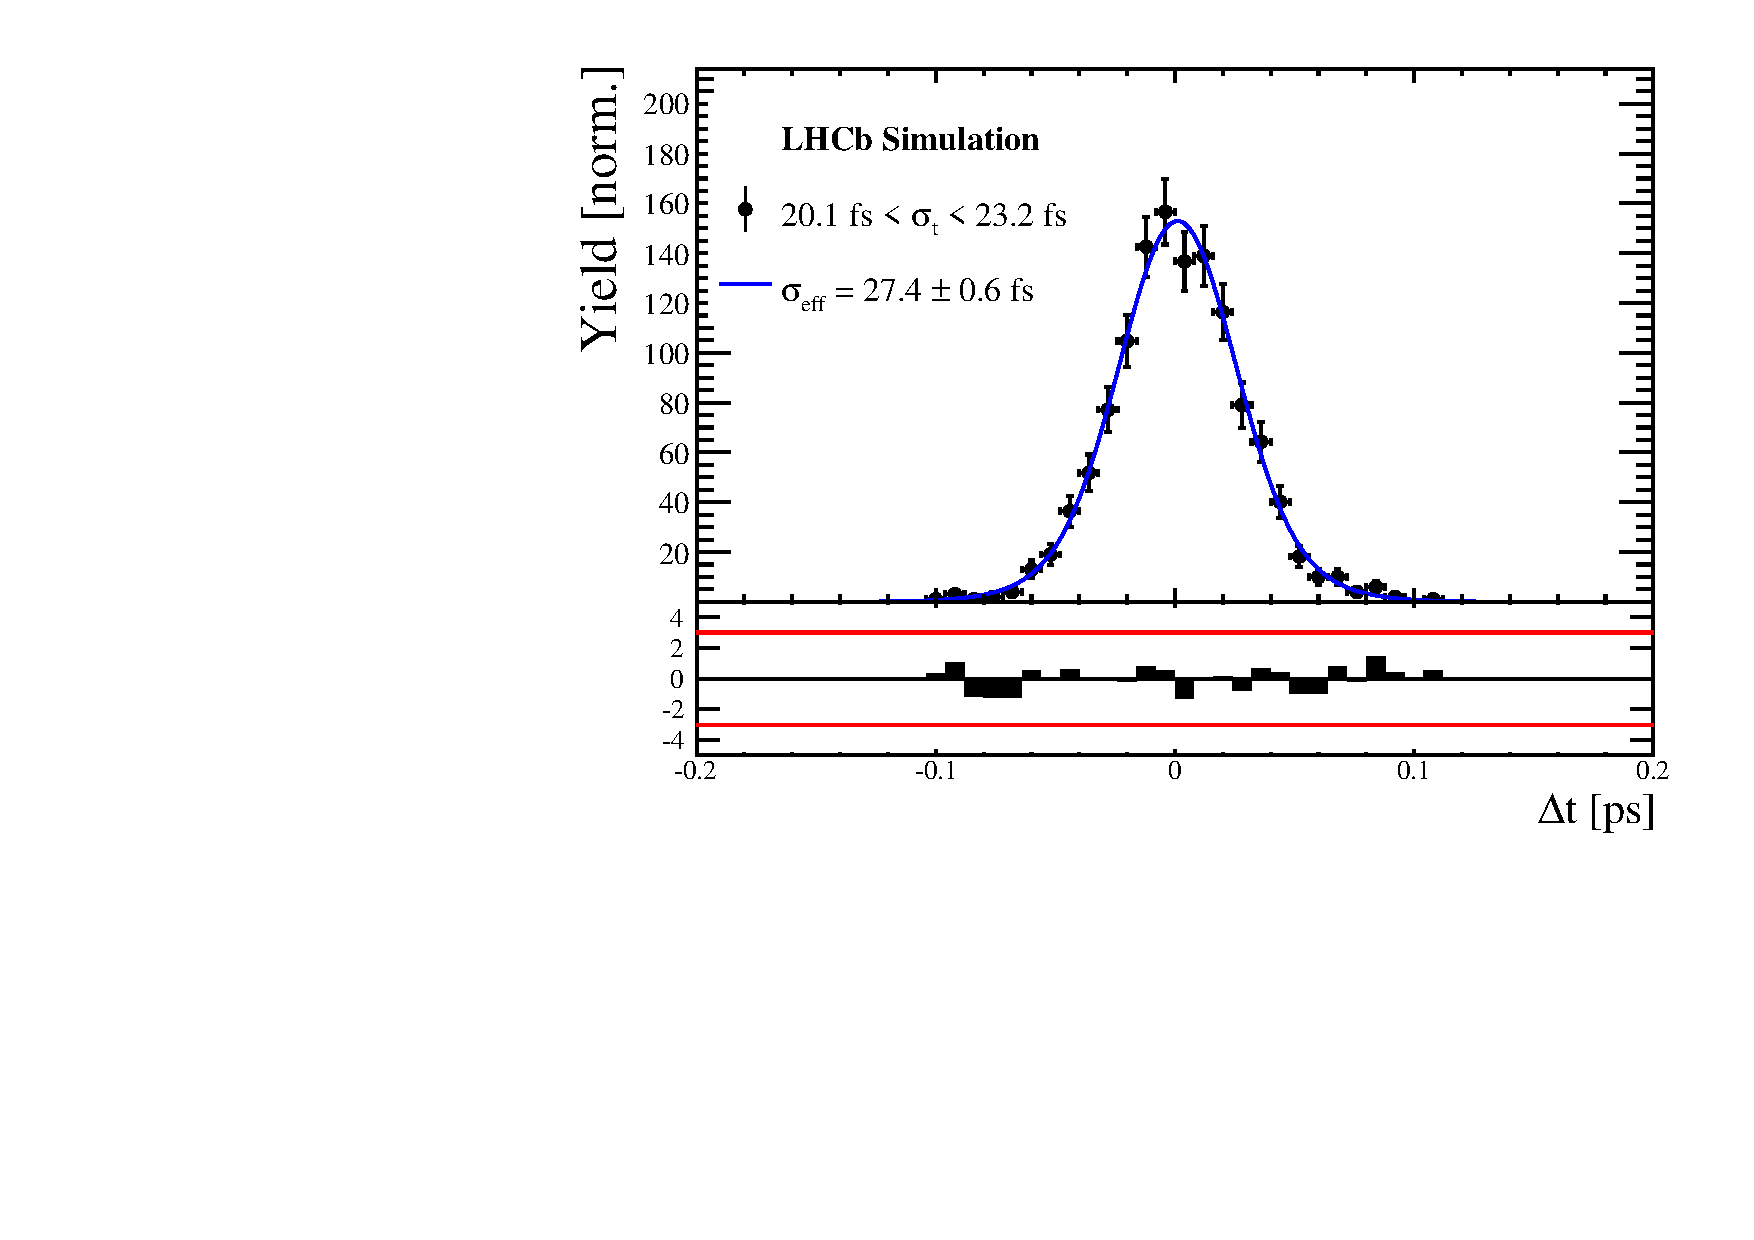
\includegraphics[height=7.4cm,width=0.7\textwidth]{figs/Resolution/SignalMC_bin_2.pdf}
\caption{Difference of the true and measured decay time of $\Bs\to\Ds\kaon\pion\pion$ candidates from MC in the bin $20.7\ps$ $<$ $\sigma_{t}$ $<$ $24.3\ps$. A fit of the sum of two Gaussian functions is overlaid.}
\label{fig:ResoFit_24to29}
\end{figure}


For the combination of the two separate widths $\sigma_{1}$ and $\sigma_{2}$, a method which takes the damping effect of the finite time resolution on the CP observables into account, is used.
The effective damping of the CP amplitudes is described by the dilution $\mathcal{D}$, which can take values between 1 and 0. 
In the case of infinite precision, there would be no damping and therefore  $\mathcal{D} = 1$ would hold, while for a resolution that is much larger than the $\Bs$ oscillation frequency, $\mathcal{D}$ would approach 0.
For two Gaussians describing the resolution, the dilution can be defined as \cite{Aaij:2017lff}

\begin{equation}
\mathcal{D} = f_{1}e^{-\sigma_{1}^{2}\dms^{2}/2} + (1 - f_{1}) e^{-\sigma_{2}^{2}\dms^{2}/2},
\label{eq:t-dilution}
\end{equation}   

where $f_{1}$ is the fraction of events described by the first Gaussian relative to the second and $\dms$ is the oscillation period of the $\Bs$ meson. \newline   
The dilution is computed in every bin of the per-event decay time error and can be converted into the effective resolution

\begin{equation}
\sigma_{eff} = \sqrt{(-2/\dms^{2})\ln{\mathcal{D}}}.
\label{eq:effres}
\end{equation}




\subsection{Results}

The fitted values for the Gaussian widths $\sigma_{1}$ and $\sigma_{2}$, 
the fraction of the first relative to the second Gaussian function $f_{1}$, as well as the effective resolution $\sigma_{eff}$, found in each bin $\sigma_{t}$, are shown in Tab. \ref{table:ResoParams}.
Figure \ref{fig:ResoFit_compared} shows the obtained values for $\sigma_{eff}$ as a function of the per-event decay time error $\sigma_{t}$. A linear polynom of the form  

\begin{equation}
\sigma(\sigma_{t})_{mc} = s_{0} + s_{1}\cdot \sigma_{t} 
\label{eq:resfit}
\end{equation}

is used to parametrise this distribution. The obtained values are 

\begin{equation}
\sigma(\sigma_{t})_{mc} = 0 + (1.257 \pm 0.017) \sigma_{t},
\label{eq:resfitres}
\end{equation}

where $s_{0}$ is compatible with 0 in the fit and therefore is set to $s_{0} = \sigma(\sigma_{t} = 0) = 0$. 
For comparison, the linear scaling functions found for $\sigma(\sigma_{t})$ in the $\Bs\to\Ds\kaon$ analysis \cite{Aaij:2017lff} for MC is also shown in Figure \ref{fig:ResoFit_compared}.  
%We introduce a correction factor to account for possible differences between the decay time resolution found in simulation and data. 
Motivated by the similarity between the $\Bs\to\Ds\kaon\pion\pion$ and $\Bs\to\Ds\kaon$ decay, we assume a comparable scaling relation for data, 

\begin{equation}
\frac{\sigma(t)_{\Ds\kaon\pion\pion,data}}{\sigma(t)_{\Ds\kaon\pion\pion,mc}} \approx  \frac{\sigma(t)_{\Ds\kaon,data}}{\sigma(t)_{\Ds\kaon,mc}}.
\label{eq:resoMCvsData}
\end{equation}

This leads to a correction factor 

\begin{equation}
\sigma(t)_{\Ds\kaon\pion\pion,data} \approx  \frac{\sigma(t)_{\Ds\kaon,data}}{\sigma(t)_{\Ds\kaon,mc}} \cdot \sigma(t)_{\Ds\kaon\pion\pion,mc},
\label{eq:resoMCvsData_2}
\end{equation}

where all elements of the right side of the equation are known. \newline

Taking the scaling function found in our simulation, as well as input from the $\Bs\to\Ds\kaon$ analysis for $\sigma(t)_{\Ds\kaon,mc/data}$, we find

\[\sigma(t)_{\Ds\kaon\pion\pion,data} = 10.3 fs + 1.28 \cdot t\],

which is the scaling factor used for the per-event decay time error in the nominal time- and amplitude-dependent fit. 


\begin{table}[h]
\centering
 \begin{tabular}{l || l l l | l l}
$\sigma_{t}$ Bin [fs] & $\sigma_{1}$ [fs] & $\sigma_{2}$ [fs] & $f_{1}$ & D & $\sigma_{eff}$ [fs] \\
\hline
0to19 & 22.57 $\pm$ 0.96 & 45.57 $\pm$ 4.061 & 0.827 $\pm$ 0.057 & 0.89 $\pm$ 0.067 & 27.46 $\pm$ 8.82 \\
19to24 & 24.64 $\pm$ 1.03 & 46.65 $\pm$ 3.109 & 0.768 $\pm$ 0.061 & 0.86 $\pm$ 0.070 & 30.64 $\pm$ 8.48 \\
24to29 & 30.96 $\pm$ 0.90 & 58.76 $\pm$ 5.684 & 0.884 $\pm$ 0.045 & 0.83 $\pm$ 0.05 & 34.66 $\pm$ 5.28 \\
29to34 & 35.28 $\pm$ 1.54 & 57 $\pm$ 6.698 & 0.839 $\pm$ 0.098 & 0.79 $\pm$ 0.10 & 39.09 $\pm$ 10.47 \\
34to39 & 37.05 $\pm$ 2.36 & 61.98 $\pm$ 5.769 & 0.707 $\pm$ 0.12 & 0.73 $\pm$ 0.12 & 44.76 $\pm$ 11.78 \\
39to44 & 68.38 $\pm$ 8.33 & 42.15 $\pm$ 3.583 & 0.331 $\pm$ 0.18 & 0.66 $\pm$ 0.16 & 50.98 $\pm$ 15.11 \\
44to49 & 199.9 $\pm$ 100.1 & 53.72 $\pm$ 1.419 & 0.020 $\pm$ 0.014 & 0.62 $\pm$ 0.02 & 54.89 $\pm$ 1.60 \\
49to150 & 68.75 $\pm$ 165.3 & 68.92 $\pm$ 4.603 & 0.001 $\pm$ 0.97 & 0.47 $\pm$ 0.65 & 68.92 $\pm$ 63.42 \\
\hline
\end{tabular}
\caption{Summary of the obtained parameters from the resolution fits described above.}
\label{table:ResoParams}
\end{table}


\begin{figure}[h]
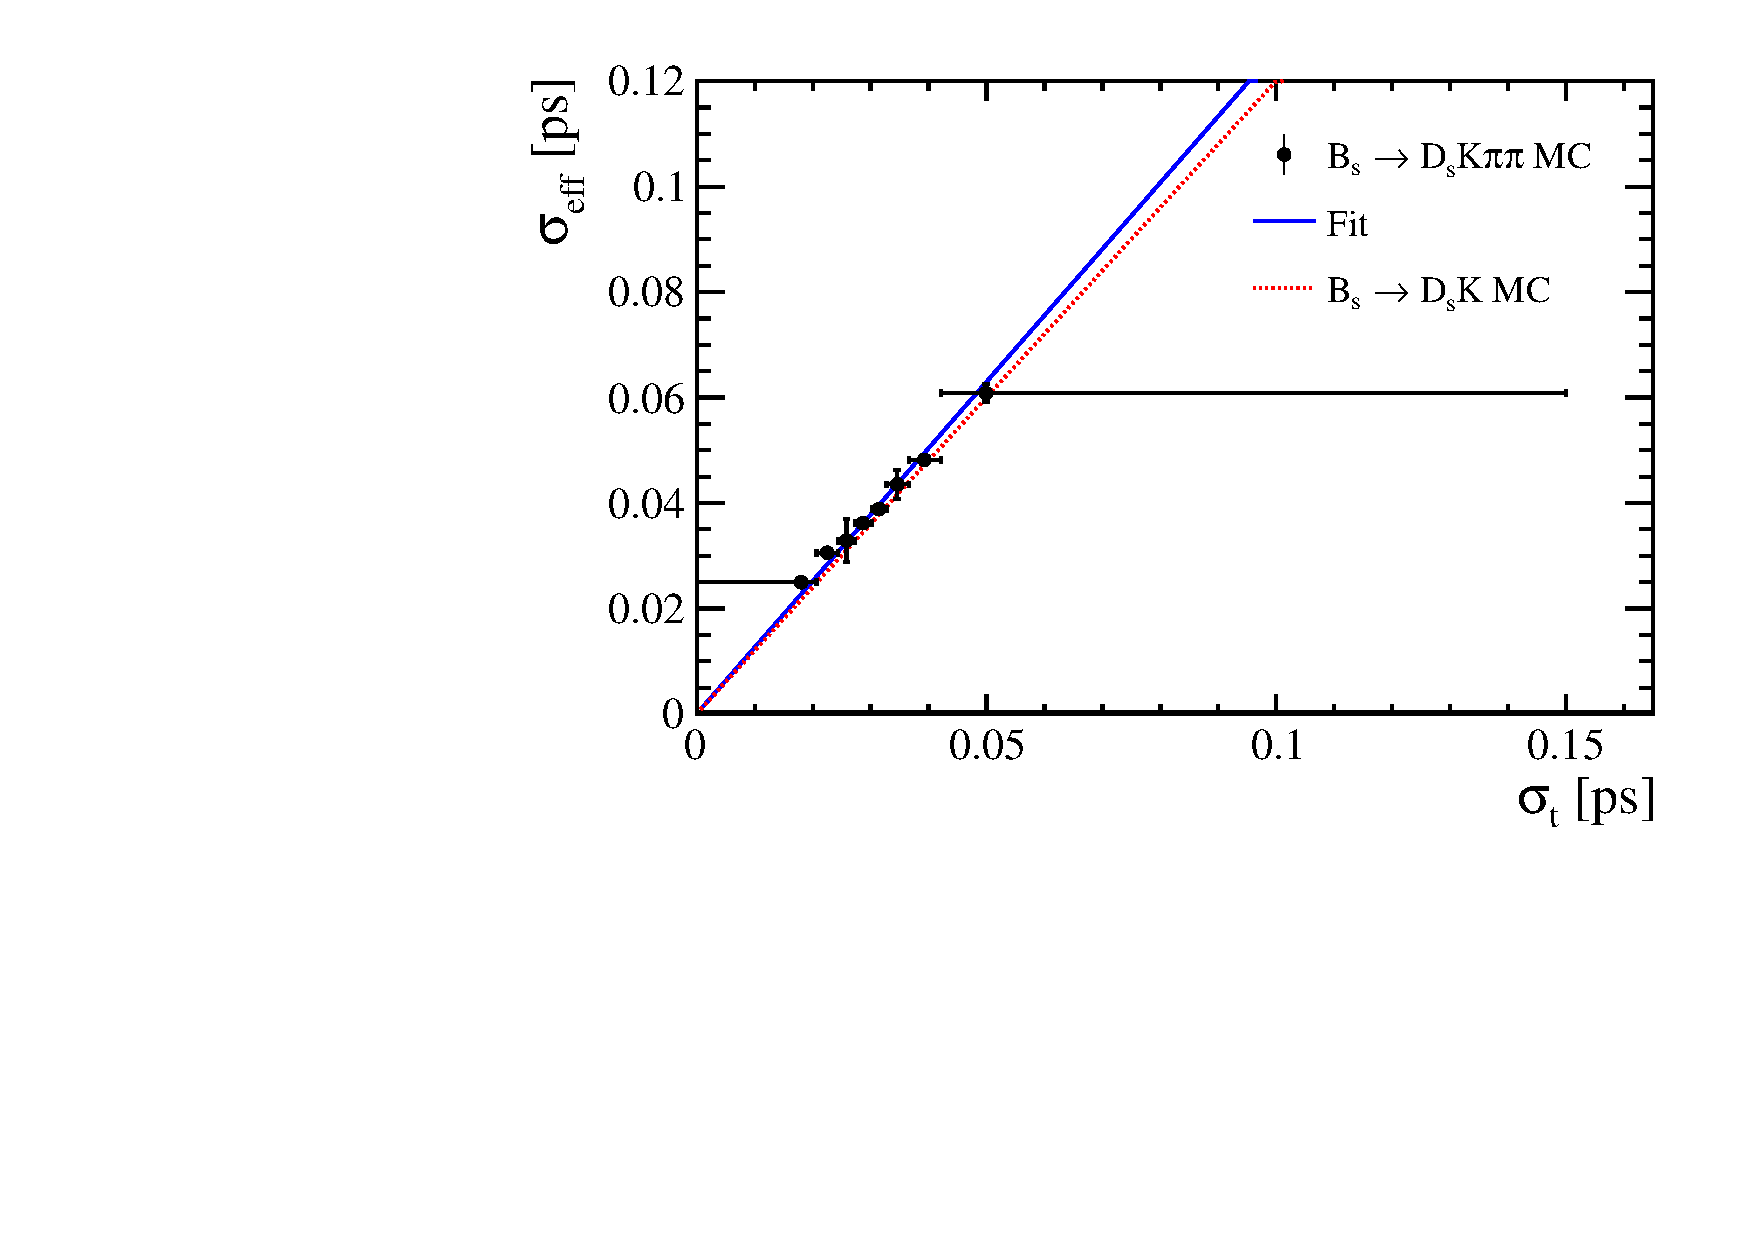
\includegraphics[height=7.4cm,width=0.7\textwidth]{figs/Resolution/ProperTimeReso_MC.pdf}
\caption{Decay-time resolution of $\Bs\to\Ds\kaon\pion\pion$ candidates from MC. 
The scaling functions found in $\Bs\to\Ds\kaon$ (dotted red line) MC is also shown for comparison. The fit described in the text is overlaid.}
\label{fig:ResoFit_compared}
\end{figure}



